% \documentclass{article}
% \usepackage[margin=1cm]{graphicx} % Required for inserting images
% \usepackage[russian]{babel}
% \usepackage{caption}
% \usepackage{geometry}
% \usepackage{url}
% \usepackage{amsfonts}
% \usepackage{amsmath}
% \usepackage{float}
% \usepackage[a4paper, top=2cm, bottom=3cm, left=3cm, right=1cm]{geometry}
\documentclass[a4paper,12pt]{article}
\usepackage[utf8]{inputenc}
\usepackage[russian]{babel}
\usepackage{amsmath}
\usepackage{multicol}
\usepackage{url}
\usepackage[margin=1cm]{graphicx} % Required for inserting images
\usepackage[a4paper, top=2cm, bottom=3cm, left=1cm, right=2cm]{geometry}

\title{Санкт-Петербургский политехнический университет
Петра Великого
Физико-механический институт
Высшая школа прикладной математики и вычислительной
физики}
\date{}
\begin{document}

\maketitle
\begin{center}
{\fontsize{25}{}\selectfont Отчёт \\
по лабораторной работе №4 \\
по дисциплине \\
«Интервальный анализ»}

\end{center}
\begin{flushright}
Выполнил студент:\\
Басалаев Даниил
группа:\\
5030102/10201\\

\end{flushright}

\vspace*{\fill} \begin{center}Санкт-Петербург\end{center}

\newpage % Начать новую страницу для содержания
\tableofcontents
\newpage

\section{Теоретическое обоснование}
Перед использованием измерительной системы её необходимо откалибровать.\\
В конечном счёте калибровка сводится к определению параметров линейной регрессии
\begin{equation}
    \textbf{y} = \mbf{\beta}_0 + \mbf{\beta}_1 \cdot \textbf{x}, 
\end{equation}
где $ \textbf{x}$ --- входные данные, $\textbf{y}$ --- выходные данные, $\mbf{\beta}_0$,  $\mbf{\beta}_1$ --- параметры регрессии.

\begin{figure}[hbt]
	\centering\normalsize
	\setlength{\unitlength}{1mm}
	\begin{picture}(90,29)
	\put(30,6){\line(1,0){30}}
	\put(30,26){\line(1,0){30}}
	\put(30,6){\line(0,1){20}}
	\put(60,6){\line(0,1){20}}
%	\put(39.5,0){$F(a,x)$}
	\put(20,12){\vector(1,0){10}}
	\put(20,20){\vector(1,0){10}}
	\put(60,12){\vector(1,0){10}}
	\put(60,20){\vector(1,0){10}}	
  \put(-5,16){ВХОДЫ}	 \put(78,16){ВЫХОДЫ}	
	\put(15,15){$x$}\put(-3,24){эталонный сигнал}
	\put(72,15){$\mbf{y}$}\put(63,24){результат измерения}
	\put(40,17.5){$\{ \mbf{\beta}_0, \mbf{\beta}_1 \}$}
 	\put(40,12.5){$8 \times 1024$}
	\end{picture}
	\caption{Структурная схема калибровки сигнала} 
	\label{f:CalibrationSystem} 
\end{figure}\\
\hspace{-0.5cm}Параметры регрессии определяются из решения \index{интервальная система линейных алгебраических уравнений, ИСЛАУ} \emph{интервальной системы линейных алгебраических уравнений}.
\begin{equation} \label{ISLAU}
    \textbf{Y} = \mbf{\beta}_0 + \mbf{\beta}_1 \cdot \textbf{X}.
\end{equation}
где $ \textbf{X}$ --- вектор входных калибровочных данных, $\textbf{Y}$ --- вектор выходных данных.\\\\
В общем случае входных данных получение  оценок параметров регрессии является нетривиальной задачей. Внешние оценки часто получаются очень грубыми. Внутренние оценки не являются однозначными и их вычисление является математически трудной задачей. Одновременное получение внутренних и внешних оценок мотивирует использование твинной арифметики. На этом пути получено еще не много результатов. 

\section{Постановка задачи}
Определить параметры линейной регрессии
$$\boldsymbol{y} = \mbf{\beta}_0 + \mbf{\beta}_1 \cdot \boldsymbol{x}, $$
где $ \textbf{x}$ --- входные данные, $\textbf{y}$ --- выходные данные, $\mbf{\beta}_0$,  $\mbf{\beta}_1$ --- параметры регрессии.\\\\
Для калибровки измерителя, на вход подаётся набор постоянных
напряжений
$$X = \{x_i\}$$
Для надёжности, для каждого значения $x$ проводится 100 измерений.\\\\
Получается набор интервальных выборок.\\
$$\boldsymbol{Y} = \{y_k\}_{k=1}^{100}$$
rad \textbf{y} = $\frac{1}{2^N}$V(В), $N=14$\\\\
\\\textbf{Файлы данных:}\\\\
27\_08\_2024ADC\_rawData.zip\\
Формат файлов — Save to BIN.pdf.\\\\
Связь кодов данных и Вольт:\\

$V = Code/16384 − 0.5$ \\

\textbf{Задание:}
\begin{enumerate}
    \item Сделать оценки значений $\boldsymbol{Y}$ двумя способами:
        \begin{itemize}
            \item in: как интервал между первым и третьим квартилем
            \item ex: как границы бокс-плота
        \end{itemize}
    \item Решить ИСЛАУ (1) для внутренних и внешних оценок $y$
    \item Построить множество решений $\mbf{\beta}_0$,  $\mbf{\beta}_1$
    \item Построить коридор совместных зависимостей
    \item Пример — https://github.com/szhilin/octave-interval-examples/blob/master/SteamGenerator.ipynb
\end{enumerate}

\newpage
\section{Результат}
\subsection{Вид данных}\\
\begin{figure}[h!]
    \centering
    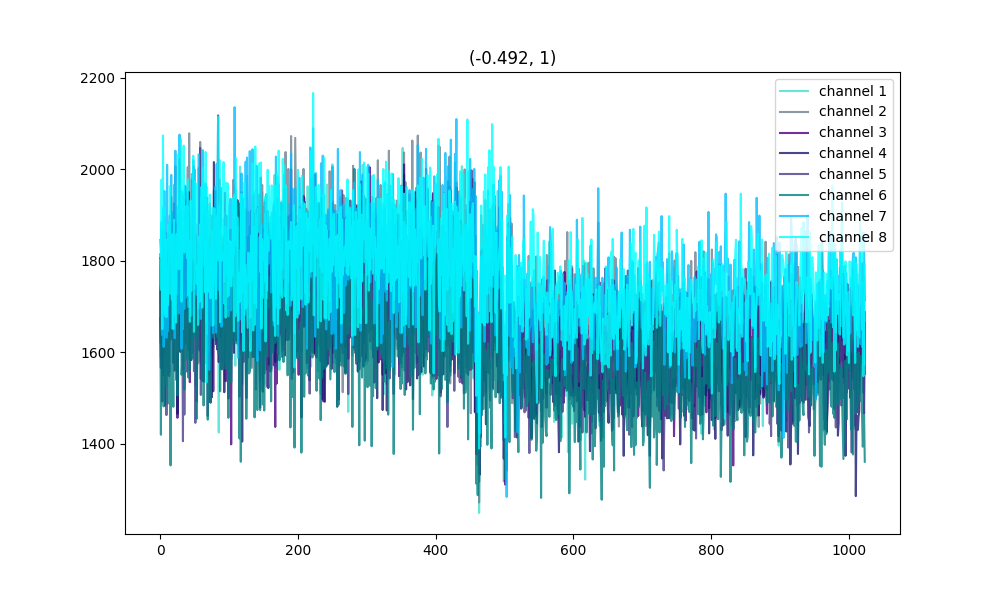
\includegraphics[width=1\linewidth]{Исходные данные.png}
    \caption{Данные для уровня -0.492, 1 канала}
\end{figure}\\
Видим по графикам, что в данных есть выбросы, их можно отсеять с помощью боксплота. Для внешних оценок возьмем границы боксплота (после отсеивания выбросов берем минимум и максимум) с параметром k=1.5, а для внутренних 1-й и 3-й квартили:

\begin{center}
\begin{tabular}{|c|c|c|}
\hline
\multicolumn{2}{|c|}{Невязка для каждого уравнения}\\
\hline
Номер уравнения&Невязка\\
\hline
1&-1.43113470e-04\\
\hline
2&6.29744978e-04\\
\hline
3&-1.43918682e-04\\
\hline
4&4.55355788e-04\\
\hline
5&4.18357459e-04\\
\hline
6&-1.24125311e-04\\
\hline
7&4.35558883e-04\\
\hline
8&-1.43342837e-04
\end{tabular}
\end{center}\\

Замечаем, что имеется 4 уравнения с отрицательной невязкой. Это говорит о том, что ИСЛАУ для неизвестных коэффициентов регресии несовместна. Для того, чтобы получить множество внутренних оценок, заменим строки системы с отрицательной невязкой (неомера уравнений будут номерами образующих распознающего функционала с отрицательным значением Tol'a)

\newpage
\subsection{Построение допускового множества}\\
Выберем для демонстрации работы алгоритма канал и ячейку - channel = 5, cell = 512
\begin{figure}[h!]
    \centering
    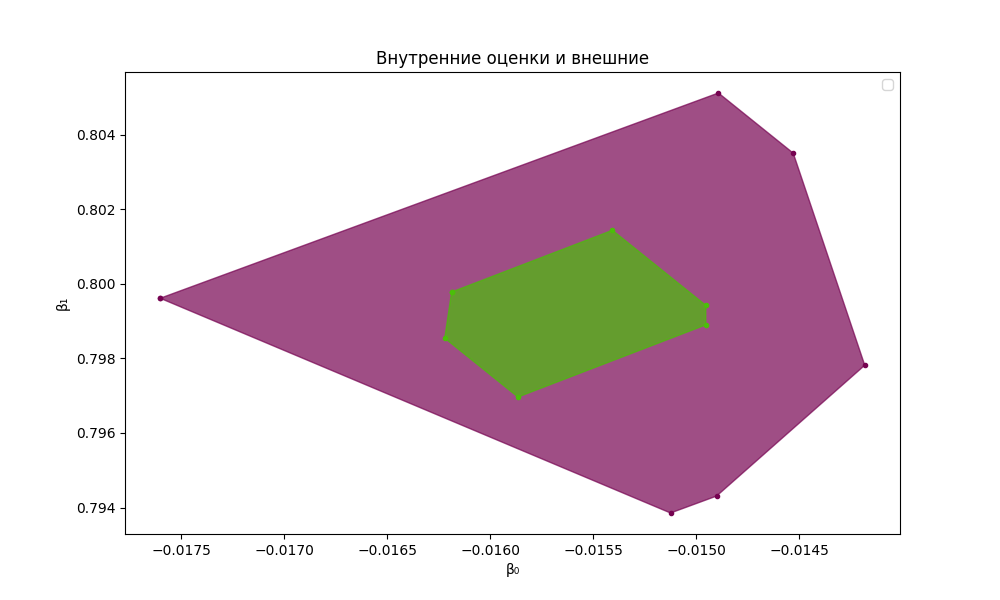
\includegraphics[width=1\linewidth]{tol-after-alg.png}
    \caption{Допусковое множество до раширения внутренних оценок до внешних}
\end{figure}

\begin{center}
\begin{tabular}{|c|c|c|}
\hline
\multicolumn{2}{|c|}{Невязка для каждого уравнения}\\
\hline
Номер уравнения&Невязка\\
\hline
1&2.36906137e-03\\
\hline
2&6.29388677e-04\\
\hline
3&1.62245122e-03\\
\hline
4&6.28479464e-04\\
\hline
5&6.28316799e-04\\
\hline
6&1.33377549e-03\\
\hline
7&7.18856272e-04\\
\hline
8&1.71299069e-03
\end{tabular}
\end{center}\\

Невязки стали положительными, а значит система стала совместной \\

\newpage
\subsection{Коридор решений}\\
\begin{figure}[h!]
    \centering
    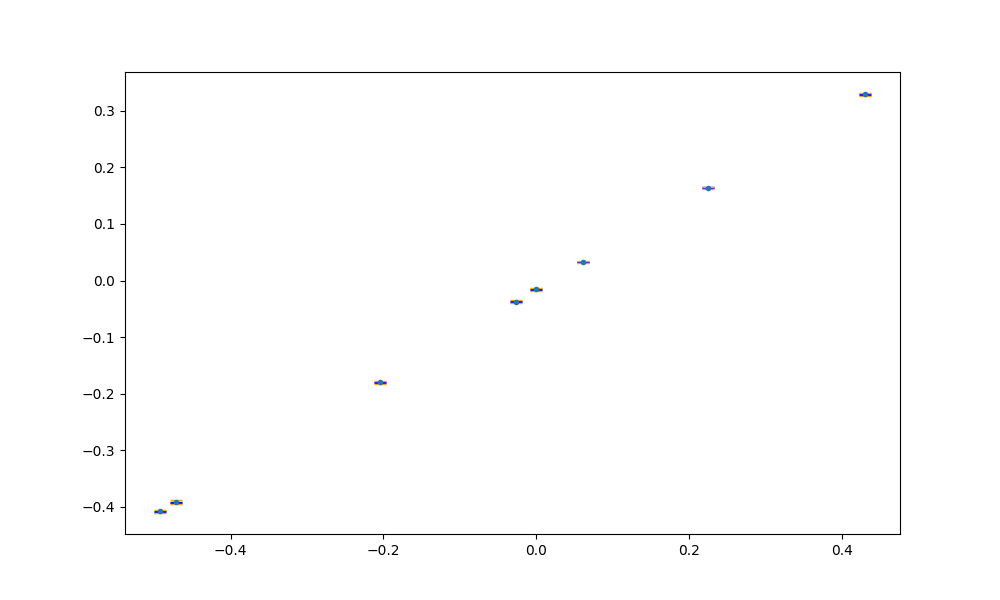
\includegraphics[width=0.8\linewidth]{intervals.png}
    \caption{Внешние и внутренние оценки границы}
\end{figure}
\begin{figure}[h!]
    \centering
    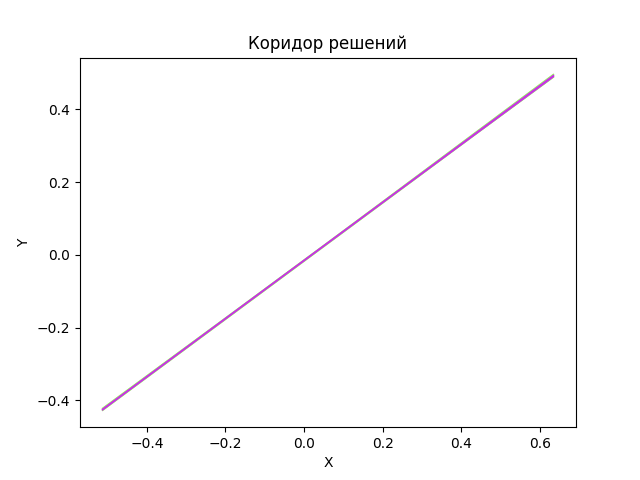
\includegraphics[width=0.8\linewidth]{Коридоры.png}
    \caption{Коридор значений}
\end{figure}
\begin{figure}[h!]
    \centering
    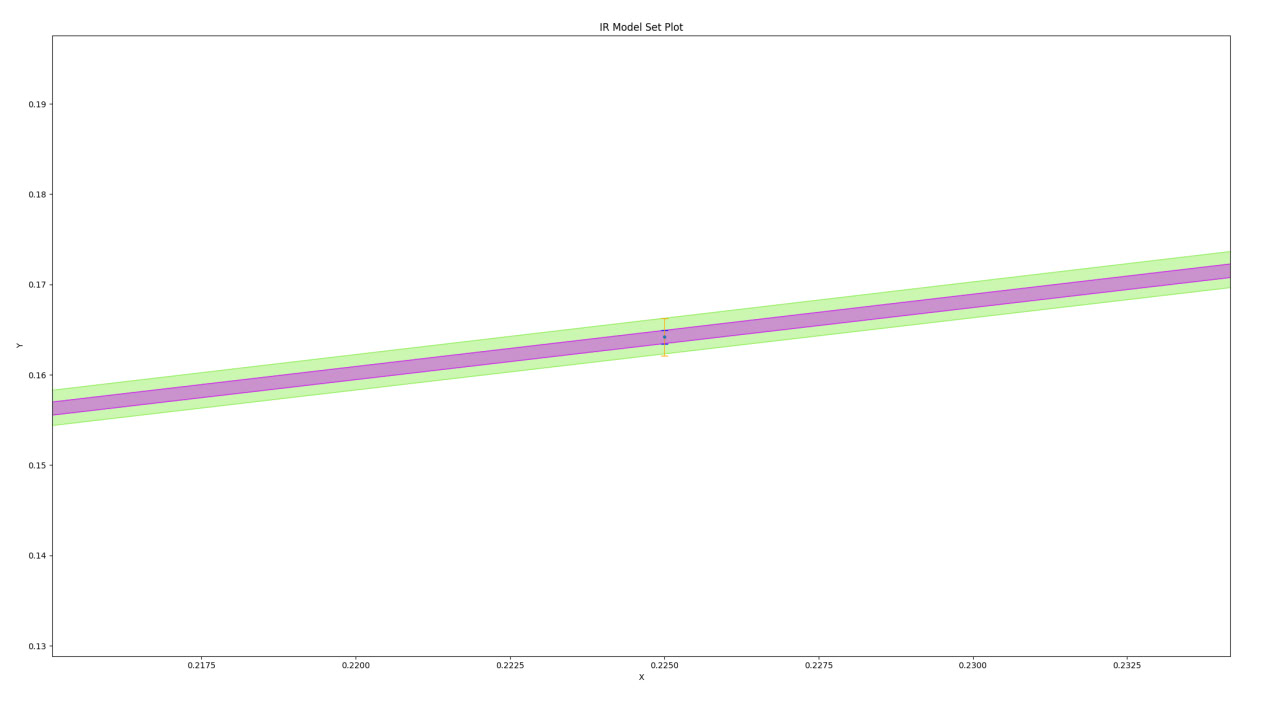
\includegraphics[width=1\linewidth]{Корридор_приближенно.jpg}
    \caption{Коридор значений в приближении}
\end{figure}

\newpage
\section{Выводы}
  В ходе выполнения лабораторной работы была реализована методика оценки
  параметров линейной регрессии на основе интервальных данных. Основные
  результаты включают в себя:

  \begin{itemize}
    \item Разработан алгоритм для нахождения внутренних и внешних оценок
      параметров линейной регрессии, что позволяет учитывать
      неопределённость в данных.
    \item Получены интервальные оценки параметров \( \beta_0 \) и
      \( \beta_1 \), которые демонстрируют диапазон возможных значений
      параметров регрессии.
    \item Построены коридоры совместных зависимостей, которые
      визуализируют интервальные решения и помогают в анализе устойчивости
      модели.
  \end{itemize}\\
  Результаты показывают, что предложенный подход позволяет более точно
  моделировать зависимости в данных, учитывая возможные вариации и ошибки.
  Это особенно полезно в приложениях, где точность измерений может
  варьироваться, и требуется надёжная оценка параметров модели.
\section{Литература}
\begin{enumerate}
    \item A.Н.Баженов. Интервальный анализ. Основы теории и учебные примеры. СПБПУ. 2020
    \item Официальная документация intvalpy: \url{https://intvalpy.readthedocs.io/ru/latest/#} 
    \item A.Н.Баженов., Н.В.Ермаков. Малоракурсная томография. Спб.: Политех-Пресс. 2023.  
\end{enumerate}

\section{GitHub}
Ссылка на репозиторий с кодом: \url{https://github.com/11AgReS1SoR11/Interval.git} \\

\section{Литература}
\begin{enumerate}
    \item A.Н.Баженов. Интервальный анализ. Основы теории и учебные примеры. СПБПУ. 2020
    \item A.Н.Баженов., Н.В.Ермаков. Малоракурсная томография. Спб.: Политех-Пресс. 2023.  
\end{enumerate}

\end{document}
